% ============================================================================================
% This is a LaTeX template used for the course
%
%  I M A G E   B A S E D   B I O M E T R I C S
%
% Faculty of Computer and Information Science
% University of Ljubljana
% Slovenia, EU
%
% You can use this template for whatever reason you like.
% If you have any questions feel free to contact
% ziga.emersic@fri.uni-lj.si
% ============================================================================================

\documentclass[9pt]{IEEEtran}

% basic
\usepackage[english]{babel}
\usepackage{graphicx,epstopdf,fancyhdr,amsmath,amsthm,amssymb,url,array,textcomp,svg,listings,hyperref,xcolor,colortbl,float,gensymb,longtable,supertabular,multicol,placeins}

 % `sumniki' in names
\usepackage[utf8x]{inputenc}

 % search and copy for `sumniki'
\usepackage[T1]{fontenc}
\usepackage{lmodern}
\usepackage{numprint}
\input{glyphtounicode}
\pdfgentounicode=1

% tidy figures
\graphicspath{{./figures/}}
\DeclareGraphicsExtensions{.pdf,.png,.jpg,.eps}

% correct bad hyphenation here
\hyphenation{op-tical net-works semi-conduc-tor trig-gs}

% ============================================================================================

\title{\vspace{0ex} %
% TITLE IN HERE:
Ear segmentation using Mask R-CNN and Cascade R-CNN
\\ \large{Assignment \#2}\\ \normalsize{Image Based Biometrics 2021/22, Faculty of Computer and Information Science, University of Ljubljana}}
\author{ %
% AUTHOR IN HERE:
Novak Marko
\vspace{-4.0ex}
}

% ============================================================================================

\begin{document}

\maketitle

\begin{abstract}
    Mask R-CNN and Detectron2 are currently state-of-the-art solutions for one-step object detection and segmentation. This report applies the approach to ear segmentation on the AWE database~\cite{DBLP:journals/corr/EmersicSP16}. % Source code used in this report is available on GitHub~\cite{github}.
\end{abstract}

\section{Introduction}

Faster R-CNN~\cite{ren2016faster} was proposed in 2015 as a solution offering simultaneous detection and classification of objects. In 2017 an upgrade called Mask R-CNN~\cite{he2018mask} was proposed, which introduced the ability to precisely segment the target objects using pixel masks. Later the same year, Cascade R-CNN~\cite{cai2017cascade} was proposed, improving detection on smaller feature pyramid samples and overall model robustness on different sizes of inputs.

This report is based on Tensorpack~\cite{wu2016tensorpack} implementation of Mask R-CNN.

\section{Methodology}

AWE dataset comes with bounding boxes and ear masks. Each mask is split according to bounding boxes for training to get an array of one mask per instance. These masks are stored as NumPy files on start and reused on each run for faster training.

The Mask R-CNN variant chosen for this task uses ResNet101 backbone CNN, a feature pyramid network head, and a cascade wrapper around the head network. Since the problem at hand deals with the segmentation of relatively small objects (ears) on larger images, cascade should provide some improvement over plain Mask R-CNN architecture with feature pyramids. Both backbone and head networks use group normalisation, which is a normalisation technique that doesn't depend on batch size. That improves detection, as regular batch normalisation varies a lot for small batches with an inconsistent number of target objects.

The model has been trained using the training dataset containing \numprint{750} images. It's been trained over \numprint{144} epochs, totaling \numprint{72000} steps (\numprint{500} steps per epoch). Training images from AWE dataset have been randomly flipped and cropped to increase the sample size for training. Initial weights for the model have been loaded from a model pre-trained on COCO dataset.

The final training took about \numprint{15} hours on a single P100 GPU.

\section{Results}

The resulting model has been tested on \numprint{250} test (validation) images from AWE dataset. The model was able to score true matches with high confidence, making it possible to achieve \numprint{99.3}\% true positive rate at just 11 false positives (Figure~\ref{fig:roc}).

\begin{figure}[h]
    \centering
    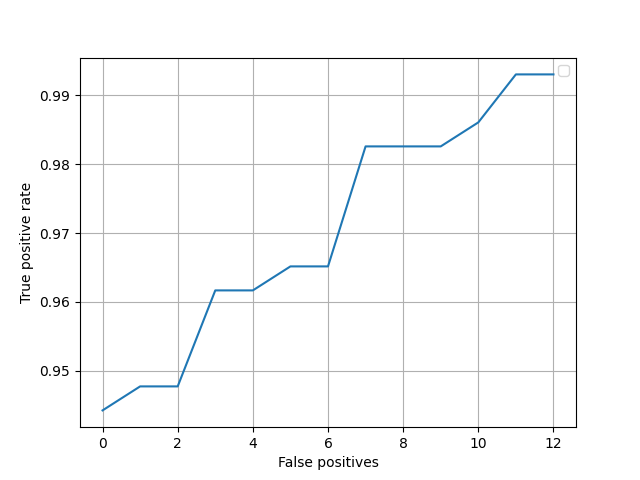
\includegraphics[width=1\columnwidth]{roc.png}
    \caption{ROC curve for the resulting model.}
    \label{fig:roc}
\end{figure}

True positive rate in realtion to false positives gives us some general idea about the performance of the model, but in order to better understand the performance of the model, additional metrics are neccesary. The following metrics were calculated based on segmentation mask:

\[ IoU = area(m_{p} \cap m_{gt}) / area(m_{p} \cup m_{gt}) \]
\[ precision = area(m_{p} \cap m_{gt}) / area(m_{p}) \]
\[ recall = area(m_{p} \cap m_{gt}) / area(m_{gt}) \]

Since false positives have small or no intersection between \(m_{p}\) (predicted mask) and \(m_{gt}\) (ground truth mask), it doesn't make sense to look at metric values relative to false positives. Instead, a confidence score from the output has been used, and a false positive count has been shown as an additional metric on the plot (figure~\ref{fig:score}).

\begin{figure}[h]
    \centering
    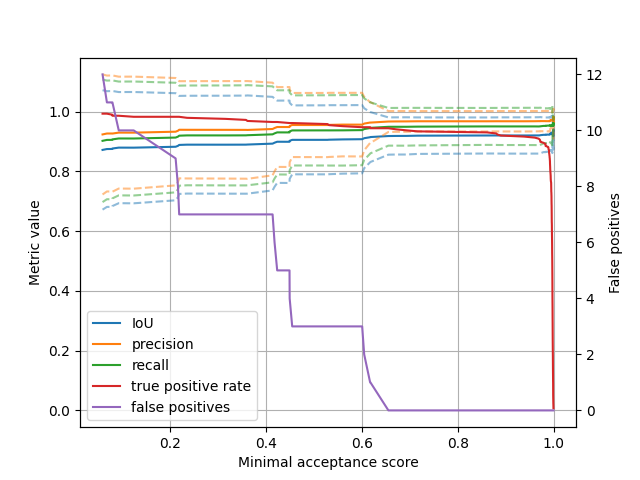
\includegraphics[width=1\columnwidth]{score.png}
    \caption{Metrics relative to minimal acceptance score.}
    \label{fig:score}
\end{figure}

The minimal acceptance score threshold of \numprint{0.65} is high enough to eliminate all false positive matches and obtain results as shown in table~\ref{tab:mean}. Using a higher threshold such as \numprint{0.90} only minimally improves the metrics but decreases true positive rate by almost \numprint{3}\%, so a larger test dataset would be needed to better determine what a good threshold value might be.

\begin{table}[hbt]
    \caption{Metric values at \(score > \numprint{0.65}\) and \(score > \numprint{0.90}\)}
    \centering
    \begin{tabular}{c | c | c | c}
        TPR & IoU & precision & recall \\
        \hline
        \numprint{94.43}\% & \shortstack{\numprint{91.85}\% \\ \pm\numprint{6.22}\%} & \shortstack{\numprint{96.67}\% \\ \pm\numprint{3.50}\%} & \shortstack{\numprint{94.91}\% \\ \pm\numprint{6.30}\%} \\
        \hline
        \numprint{91.64}\% & \shortstack{\numprint{92.02}\% \\ \pm\numprint{6.08}\%} & \shortstack{\numprint{96.77}\% \\ \pm\numprint{3.41}\%} & \shortstack{\numprint{95.03}\% \\ \pm\numprint{6.24}\%} \\
    \end{tabular}
    \label{tab:mean}
\end{table}

\section{Conclusion}

This report seems to indicate some improvement for ear detection and segmentation using Mask R-CNN over research presented in {Mask R-CNN for Ear Detection}~\cite{8756760}, which is likely due to the use of cascade wrapper and better normalisation methods. However, while both models use the same training and validation datasets, I was unable to find the exact code used to calculate the metrics in the original paper. Because of that, raw predictions data is included with the report for further analysis.

\bibliographystyle{IEEEtran}
\bibliography{bibliography}

\end{document}
